% Complex Tori and Elliptic Curves --- SYNTHESIS poster (A0 portrait).
% "One object, three faces", organized for richness: each face over C is developed with its
% core machinery -- analytic (lattice, wp, Eisenstein, periods), geometric (divisors,
% Riemann-Roch, the |3O| embedding, the Jacobian, Hodge cohomology), algebraic (the cubic,
% the group scheme, torsion, degenerations).  Column 3 specializes to a finite field for the
% arithmetic frontier.  Standalone sheet; shares figuremacros/palette.  Build x2.
\documentclass[25pt, a0paper, portrait, margin=14mm, innermargin=15mm,
               blockverticalspace=11mm, colspace=15mm, subcolspace=8mm]{tikzposter}

\usepackage{amsmath,amssymb,mathtools}

% figuremacros.tex --- figure infrastructure harvested from book/preamble.tex
% (TikZ libraries, the form* colour palette, the three \drawprecise macros,
%  and the diagram tikzset). Do not edit; mirror of the book's definitions.

\usetikzlibrary{arrows.meta,calc,positioning,decorations.markings,decorations.pathmorphing,
  patterns,shadings,shapes.geometric,fadings,backgrounds,intersections,bending}

\definecolor{formteal}{HTML}{1f4e79}
\definecolor{formgold}{HTML}{b88a14}
\definecolor{formrust}{HTML}{a8431d}
\definecolor{formplum}{HTML}{6b2e6e}
\definecolor{formsage}{HTML}{467b3a}
\definecolor{formslate}{HTML}{3a5168}
\definecolor{formivory}{HTML}{f6efe0}

\newcommand{\drawprecisetorus}{%
  % (1) Fill the visible torus body with light teal.
  \fill[formteal!13, line join=round]
    plot[smooth cycle] coordinates {\torusOuter};
  % (2) Cut out the donut hole using the inner silhouette curve.
  \fill[white, line join=round]
    plot[smooth cycle] coordinates {\torusInner};
  % (3) Visible meridian arcs (eight small circles spaced 45 deg apart).
  % Back meridians (v in [0, pi]) form one visible arc each;
  % front meridians (v in (pi, 2 pi)) wrap across u = 0 and are split
  % into two visible chunks (VA and VB) by the sampling boundary.
  \draw[draw=formteal!60!black, line width=0.42pt, line join=round, opacity=0.9]
    plot[smooth] coordinates {\torusMerZeroVA};
  \draw[draw=formteal!60!black, line width=0.42pt, line join=round, opacity=0.9]
    plot[smooth] coordinates {\torusMerOneVA};
  \draw[draw=formteal!60!black, line width=0.42pt, line join=round, opacity=0.9]
    plot[smooth] coordinates {\torusMerTwoVA};
  \draw[draw=formteal!60!black, line width=0.42pt, line join=round, opacity=0.9]
    plot[smooth] coordinates {\torusMerThreeVA};
  \draw[draw=formteal!60!black, line width=0.42pt, line join=round, opacity=0.9]
    plot[smooth] coordinates {\torusMerFourVA};
  \draw[draw=formteal!60!black, line width=0.42pt, line join=round, opacity=0.9]
    plot[smooth] coordinates {\torusMerFiveVA};
  \draw[draw=formteal!60!black, line width=0.42pt, line join=round, opacity=0.9]
    plot[smooth] coordinates {\torusMerFiveVB};
  \draw[draw=formteal!60!black, line width=0.42pt, line join=round, opacity=0.9]
    plot[smooth] coordinates {\torusMerSixVA};
  \draw[draw=formteal!60!black, line width=0.42pt, line join=round, opacity=0.9]
    plot[smooth] coordinates {\torusMerSixVB};
  \draw[draw=formteal!60!black, line width=0.42pt, line join=round, opacity=0.9]
    plot[smooth] coordinates {\torusMerSevenVA};
  \draw[draw=formteal!60!black, line width=0.42pt, line join=round, opacity=0.9]
    plot[smooth] coordinates {\torusMerSevenVB};
  % (4) Visible longitude arcs (the four canonical latitude circles).
  % Outer (u=0) is visible only on the front half (v in (pi, 2 pi)),
  % inner (u=pi) only on the back half (v in (0, pi)); the top crest
  % (u=pi/2) is visible everywhere; the bottom (u=3pi/2) is fully hidden.
  \draw[draw=formteal!60!black, line width=0.5pt, line join=round, opacity=0.95]
    plot[smooth] coordinates {\torusLonTopVA};
  \draw[draw=formteal!60!black, line width=0.42pt, line join=round, opacity=0.8]
    plot[smooth] coordinates {\torusLonOuterVA};
  \draw[draw=formteal!60!black, line width=0.42pt, line join=round, opacity=0.8]
    plot[smooth] coordinates {\torusLonInnerVA};
  % (5) Crisp silhouette outlines drawn last so they sit on top.
  \draw[draw=formteal!65!black, line width=0.95pt, line join=round]
    plot[smooth cycle] coordinates {\torusOuter};
  \draw[draw=formteal!65!black, line width=0.8pt, line join=round]
    plot[smooth cycle] coordinates {\torusInner};
}

\newcommand{\drawprecisesphere}{%
  % Color tone matches the torus (formteal) for visual unity across figures.
  % (1) Flat-filled body of the sphere (same filling style as the torus)
  \fill[formteal!13, line join=round]
    plot[smooth cycle] coordinates {\sphereOutline};
  % (2) Visible latitude arcs
  \draw[draw=formteal!60!black, line width=0.45pt, line join=round, opacity=0.9]
    plot[smooth] coordinates {\sphereLatEquatorVA};
  \draw[draw=formteal!60!black, line width=0.4pt, line join=round, opacity=0.85]
    plot[smooth] coordinates {\sphereLatNorthVA};
  \draw[draw=formteal!60!black, line width=0.4pt, line join=round, opacity=0.85]
    plot[smooth] coordinates {\sphereLatNorthVB};
  \draw[draw=formteal!60!black, line width=0.4pt, line join=round, opacity=0.85]
    plot[smooth] coordinates {\sphereLatTropicVA};
  \draw[draw=formteal!60!black, line width=0.4pt, line join=round, opacity=0.85]
    plot[smooth] coordinates {\sphereLatTropicVB};
  \draw[draw=formteal!60!black, line width=0.4pt, line join=round, opacity=0.85]
    plot[smooth] coordinates {\sphereLatSouthVA};
  % (3) Visible meridian arcs (eight meridians at v = k pi/4)
  \draw[draw=formteal!60!black, line width=0.42pt, line join=round, opacity=0.9]
    plot[smooth] coordinates {\sphereMerZeroVA};
  \draw[draw=formteal!60!black, line width=0.42pt, line join=round, opacity=0.9]
    plot[smooth] coordinates {\sphereMerOneVA};
  \draw[draw=formteal!60!black, line width=0.42pt, line join=round, opacity=0.9]
    plot[smooth] coordinates {\sphereMerTwoVA};
  \draw[draw=formteal!60!black, line width=0.42pt, line join=round, opacity=0.9]
    plot[smooth] coordinates {\sphereMerThreeVA};
  \draw[draw=formteal!60!black, line width=0.42pt, line join=round, opacity=0.9]
    plot[smooth] coordinates {\sphereMerFourVA};
  \draw[draw=formteal!60!black, line width=0.42pt, line join=round, opacity=0.9]
    plot[smooth] coordinates {\sphereMerFiveVA};
  \draw[draw=formteal!60!black, line width=0.42pt, line join=round, opacity=0.9]
    plot[smooth] coordinates {\sphereMerSixVA};
  \draw[draw=formteal!60!black, line width=0.42pt, line join=round, opacity=0.9]
    plot[smooth] coordinates {\sphereMerSevenVA};
  % (4) Hidden back arcs as dashed light strokes
  \draw[draw=formteal!50!black, dashed, line width=0.3pt, line join=round, opacity=0.55]
    plot[smooth] coordinates {\sphereLatEquatorHA};
  % (5) Crisp silhouette outline on top
  \draw[draw=formteal!65!black, line width=0.95pt, line join=round]
    plot[smooth cycle] coordinates {\sphereOutline};
}

\newcommand{\drawprecisecurve}{%
  % Oval (compact component, x in [-1,0]): draw as closed smooth cycle.
  \draw[draw=formteal!60!black, line width=0.88pt, line join=round]
    plot[smooth cycle, tension=0.85] coordinates {\curveOvalFull};
  % Branch (unbounded component, x >= 1): upper and lower arcs.
  \draw[draw=formteal!60!black, line width=0.88pt, line join=round]
    plot[smooth, tension=0.9] coordinates {\curveBranchUpper};
  \draw[draw=formteal!60!black, line width=0.88pt, line join=round]
    plot[smooth, tension=0.9] coordinates {\curveBranchLower};
  % Branch points (Weierstrass roots e1=-1, e2=0, e3=1)
  \fill[formteal!70!black] (-1,0) circle (1.8pt);
  \fill[formteal!70!black] ( 0,0) circle (1.8pt);
  \fill[formteal!70!black] ( 1,0) circle (1.8pt);
}

\tikzset{
  arrow/.style={-{Latex[length=2mm]}, thick},
  point/.style={circle, fill=black, inner sep=1.5pt},
  labelnode/.style={font=\small, align=center},
  note/.style={draw=black!55, rounded corners=2pt, align=center, inner sep=5pt, fill=black!3},
  visualnode/.style={draw=black!60, rounded corners=2pt, align=center, inner sep=6pt, fill=black!2}
}


\newcommand{\C}{\mathbb{C}}
\newcommand{\R}{\mathbb{R}}
\newcommand{\Z}{\mathbb{Z}}
\newcommand{\Q}{\mathbb{Q}}
\newcommand{\F}{\mathbb{F}}
\newcommand{\CP}{\mathbb{CP}}
\newcommand{\HH}{\mathbb{H}}
\newcommand{\Pic}{\operatorname{Pic}}
\newcommand{\Div}{\operatorname{Div}}
\newcommand{\ord}{\operatorname{ord}}
\newcommand{\Jac}{\operatorname{Jac}}
\newcommand{\divisor}{\operatorname{div}}

\newcommand{\sagedir}{../sagemath}
\input{\sagedir/coords.tex}
\input{\sagedir/coords_torus.tex}
\input{\sagedir/coords_curve_sample.tex}

\definecolorstyle{book}{}{%
  \colorlet{backgroundcolor}{formivory!55}%
  \colorlet{framecolor}{formteal!70!black}%
}{%
  \colorlet{titlefgcolor}{formivory}%
  \colorlet{titlebgcolor}{formteal!88!black}%
}{%
  \colorlet{blocktitlebgcolor}{formteal}%
  \colorlet{blocktitlefgcolor}{white}%
  \colorlet{blockbodybgcolor}{white}%
  \colorlet{blockbodyfgcolor}{black}%
}{%
  \colorlet{innerblocktitlebgcolor}{formgold}%
  \colorlet{innerblocktitlefgcolor}{black}%
  \colorlet{innerblockbodybgcolor}{formgold!18}%
  \colorlet{innerblockbodyfgcolor}{black}%
}{%
  \colorlet{notefgcolor}{black}%
  \colorlet{notebgcolor}{formgold!22}%
  \colorlet{notefrcolor}{formgold!80!black}%
}
\usetheme{Default}
\usecolorstyle{book}

\newcommand{\figH}[2]{\par\smallskip{\centering\resizebox{!}{#1}{#2}\par}\smallskip}
\newcommand{\figcap}[1]{{\centering\small\itshape #1\par}\smallskip}
\newcommand{\callout}[3]{%
  \par\medskip\noindent
  \begin{tikzpicture}
    \node[fill=#1!17, draw=#1!80!black, line width=1.1pt, rounded corners=6pt,
          inner sep=11pt, text width=\dimexpr\linewidth-38pt\relax, align=left]
      {\textbf{#2}\, #3};
  \end{tikzpicture}\par\medskip}

\title{Complex Tori and Elliptic Curves}
\author{One Object, Three Faces --- over $\C$}
\institute{The same compact complex Lie group as a torus $\C/\Lambda$, a Jacobian $\Pic^0(E)$, and a curve $E(\C)$}
\makeatletter
\settitle{%
  \centering\color{titlefgcolor}%
  {\fontsize{56}{64}\selectfont\bfseries \@title}\\[0.28em]
  {\fontsize{34}{40}\selectfont\bfseries \@author}\\[0.16em]
  {\fontsize{22}{27}\selectfont\itshape \@institute}%
}
\makeatother

\begin{document}
\maketitle[width=\textwidth]

% ===================== HEADER: thesis + trinity =====================
\block{\large One Object, Three Faces, over $\C$}{%
\normalsize
\begin{minipage}[c]{0.40\linewidth}
A single object --- a compact one-dimensional complex Lie group, a \emph{one-dimensional
abelian variety} --- appears in three guises: the torus $\C/\Lambda$ (analytic), the
Jacobian $\Pic^0(E)$ (geometric), the projective curve $E(\C)$ (algebraic).
\textbf{Uniformization makes all three one group}, by explicit biholomorphisms. Columns 1--2
develop each face; column 3 specializes the field to $\F_p$ for the arithmetic frontier.
\callout{formteal}{The thesis.}{$\C/\Lambda\cong\Pic^0(E)\cong E(\C)$ as complex Lie
groups; analysis, geometry, and algebra describe \emph{one} object.}
\end{minipage}\hfill
\begin{minipage}[c]{0.57\linewidth}
{\centering\resizebox{0.99\linewidth}{!}{% The TRINITY: one abelian group seen three ways, with the isomorphisms between them.
%   analytic  C/Lambda  --Phi-->  E(k) arithmetic  --[P]-[O]-->  Pic^0(E) geometric  --s-->
% back to C/Lambda.  Every edge is an isomorphism.
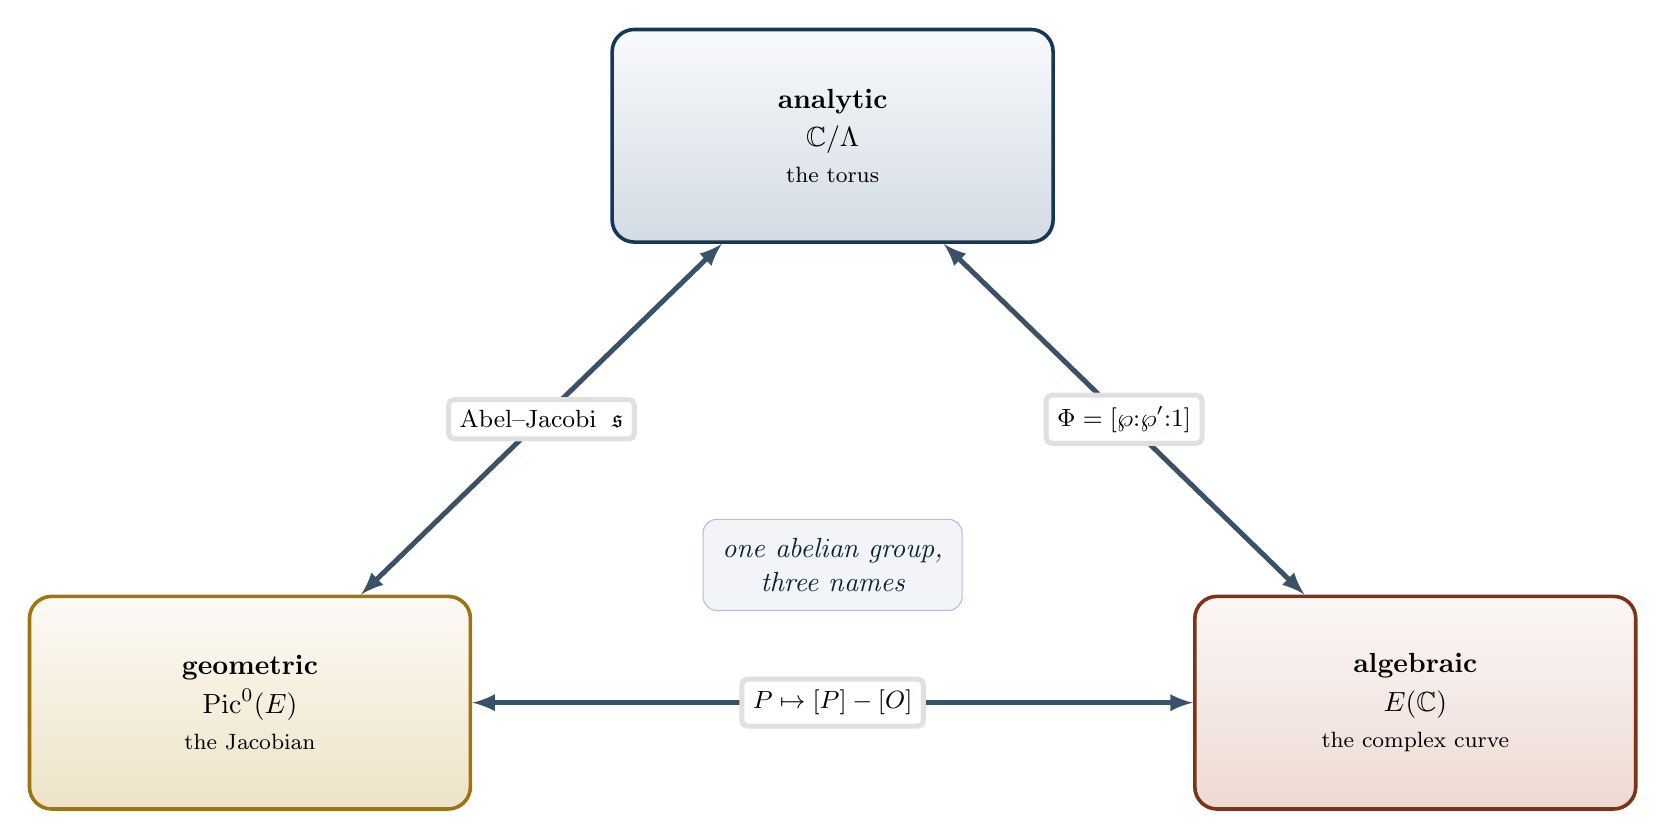
\begin{tikzpicture}[>=Latex,
    face/.style={rectangle, rounded corners=8pt, line width=1.3pt, align=center,
      inner sep=11pt, minimum width=5.6cm, minimum height=2.7cm},
    iso/.style={latex-latex, line width=1.8pt, draw=formslate},
    lbl/.style={fill=white, draw=black!12, rounded corners=2pt, inner sep=4pt,
      font=\small, align=center}]
  \node[face, draw=formteal!72!black, top color=formteal!3, bottom color=formteal!20] (an)
    at (0,7.2) {\textbf{analytic}\\[2pt]$\C/\Lambda$\\[1pt]{\footnotesize the torus}};
  \node[face, draw=formgold!85!black, top color=formgold!4, bottom color=formgold!24] (geo)
    at (-7.4,0) {\textbf{geometric}\\[2pt]$\Pic^0(E)$\\[1pt]{\footnotesize the Jacobian}};
  \node[face, draw=formrust!75!black, top color=formrust!4, bottom color=formrust!20] (ar)
    at (7.4,0) {\textbf{algebraic}\\[2pt]$E(\C)$\\[1pt]{\footnotesize the complex curve}};
  \draw[iso] (an) -- node[lbl] {$\Phi=[\wp{:}\wp'{:}1]$} (ar);
  \draw[iso] (ar) -- node[lbl] {$P\mapsto[P]-[O]$} (geo);
  \draw[iso] (geo) -- node[lbl] {Abel--Jacobi $\;\mathfrak{s}$} (an);
  \node[draw=formteal!35, fill=formteal!6, rounded corners=5pt, inner sep=7pt,
        align=center, font=\itshape, text=formteal!45!black] at (0,1.75)
    {one abelian group,\\ three names};
\end{tikzpicture}
}\par}
{\centering\small\itshape The maps: $\Phi=[\wp{:}\wp'{:}1]$ (torus to cubic);
$P\mapsto[P]-[O]$ (curve to Jacobian); Abel--Jacobi $\mathfrak{s}$ (divisor to a point of
$\C/\Lambda$). Compose around the triangle and return to the start.\par}
\end{minipage}}

\begin{columns}

%========================= COLUMN 1: analytic + geometric =========================
\column{0.33}

\block{\large \textbf{1.} Analytic: the torus $\C/\Lambda$}{%
\normalsize
A \textbf{lattice} $\Lambda=\Z\omega_1+\Z\omega_2$ ($\omega_2/\omega_1\in\HH$) tiles $\C$;
$T=\C/\Lambda$ is topologically $S^1\!\times\!S^1$, a compact \textbf{genus-$1$ Riemann
surface} and a \textbf{complex Lie group}, $[u]\oplus[v]=[u+v]$.
\figH{156pt}{\begin{tikzpicture}\drawprecisetorus\end{tikzpicture}}
\figcap{$\C$ tiled by $\Lambda$, glued into the torus --- the group carried to all faces.}
\textbf{The Weierstrass function.} The simplest non-constant elliptic function,
\[ \wp(z)=\frac1{z^2}+\!\!\sum_{\lambda\neq0}\!\Big(\frac1{(z-\lambda)^2}-\frac1{\lambda^2}\Big), \]
has one double pole per cell. With the Eisenstein series $g_2=60G_4,\ g_3=140G_6$ it obeys
$\wp'^2=4\wp^3-g_2\wp-g_3$, and $\C(\wp,\wp')$ is the \emph{entire} field of elliptic
functions.
\par\smallskip
\textbf{Periods \& uniformization.} The holomorphic $1$-forms are exactly $\C\,dz$, with
$\oint_{\gamma_i}dz=\omega_i$, so $\Lambda$ is the period lattice. Conversely every genus-$1$
surface with a base point is such a $\C/\Lambda$, unique up to scaling.}

\block{\large \textbf{2.} Geometric: divisors, Riemann--Roch, $\Pic^0$}{%
\normalsize
A \textbf{divisor} $D=\sum n_i[P_i]$ has degree $\sum n_i$; principal divisors
$\divisor(f)$ have degree $0$.
\par\smallskip
\textbf{Riemann--Roch.} On genus $1$, $\ell(D)=\deg D$ for $\deg D>0$. Hence $\ell(nO)=n$,
and $1,\wp,\wp'$ span $L(3O)$ --- \emph{these are the functions that embed $E$ as a plane
cubic.}
\par\smallskip
\textbf{The Jacobian.} $\Pic^0(E)=\Div^0(E)/\{\divisor(f)\}$, the degree-$0$ line bundles.
By \textbf{Abel's theorem} (principal $\iff$ degree and sum vanish), the sum map
$\mathfrak{s}(\sum n_i[P_i])=\sum n_iz_i$ gives $\Pic^0(E)\cong\C/\Lambda$, and
$P\mapsto[P]-[O]$ makes $E$ its own Jacobian, $E\cong\Jac(E)$.
\figH{180pt}{% Abel--Jacobi: a degree-0 divisor D = (p1)+(p2)-(q1)-(q2) on E maps to the point
% s(D) = p1 + p2 - q1 - q2  of  C/Lambda.  Principal divisors map to 0 -- which is exactly
% why Pic^0(E) = C/Lambda.  (Zeros as circles, poles as crosses.)
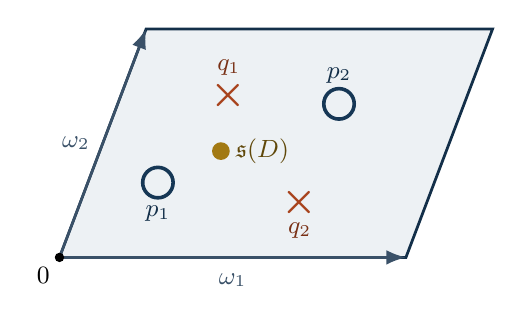
\begin{tikzpicture}[>=Latex]
  \def\ax{4.4}\def\bx{1.1}\def\by{2.9}
  \fill[formteal!8] (0,0)--(\ax,0)--(\ax+\bx,\by)--(\bx,\by)--cycle;
  \draw[formteal!60!black, line width=1pt] (0,0)--(\ax,0)--(\ax+\bx,\by)--(\bx,\by)--cycle;
  \draw[->, formslate, line width=0.9pt] (0,0)--(\ax,0) node[midway, below=2pt, font=\small] {$\omega_1$};
  \draw[->, formslate, line width=0.9pt] (0,0)--(\bx,\by) node[midway, left=1pt, font=\small] {$\omega_2$};
  % zeros (o)
  \draw[formteal!70!black, line width=1.3pt] (1.25,0.95) circle (5.5pt);
  \node[font=\small, formteal!60!black, below=5pt] at (1.25,0.95) {$p_1$};
  \draw[formteal!70!black, line width=1.3pt] (3.55,1.95) circle (5.5pt);
  \node[font=\small, formteal!60!black, above=4pt] at (3.55,1.95) {$p_2$};
  % poles (x)
  \node[formrust, font=\Large] at (2.15,2.05) {$\boldsymbol\times$};
  \node[font=\small, formrust!72!black, above=4pt] at (2.15,2.05) {$q_1$};
  \node[formrust, font=\Large] at (3.05,0.7) {$\boldsymbol\times$};
  \node[font=\small, formrust!72!black, below=4pt] at (3.05,0.7) {$q_2$};
  % the Abel sum
  \fill[formgold!88!black] (2.05,1.35) circle (3.2pt);
  \node[font=\small, formgold!52!black, right=2pt] at (2.05,1.35) {$\mathfrak{s}(D)$};
  \fill[black] (0,0) circle (1.7pt) node[below left, font=\small] {$0$};
\end{tikzpicture}
}
\figcap{Abel--Jacobi sends a degree-$0$ divisor to $\sum n_iz_i$, vanishing exactly on
principal divisors --- so $\Pic^0(E)=\C/\Lambda$.}}

%========================= COLUMN 2: algebraic + cohomology + moduli =========================
\column{0.33}

\block{\large \textbf{3.} Algebraic: the curve $E(\C)$}{%
\normalsize
The embedding $\Phi=[\wp{:}\wp'{:}1]$, $\Phi(0)=O=[0{:}1{:}0]$, is a \textbf{biholomorphism}
of $\C/\Lambda$ onto the smooth cubic $E:\,y^2=4x^3-g_2x-g_3\subset\CP^2$ --- a projective
curve of genus $1$ and a one-dimensional \textbf{abelian variety}.
\figH{160pt}{% Chord law on E: y^2 = 4x^3 - 4x, using Sage-computed chord coordinates.
\begin{tikzpicture}[scale=1.0, every node/.style={font=\small}]
  \draw[->, black!45, line width=0.5pt] (-1.7,0) -- (2.7,0) node[right, black!55] {$x$};
  \draw[->, black!45, line width=0.5pt] (0,-3.3) -- (0,3.5) node[above, black!55] {$y$};
  \drawprecisecurve
  \foreach \rt in {\rooteone,\rootetwo,\rootethree}
    \fill[formteal!60!black] (\rt,0) circle (1.4pt);
  \draw[draw=formplum, line width=0.9pt] (\chordlefta,\chordleftb) -- (\chordrighta,\chordrightb);
  \draw[dashed, line width=0.5pt, formgold!75!black] (\chordRx,\chordRy) -- (\chordSx,\chordSy);
  \fill[formrust!85!black] (\chordPx,\chordPy) circle (2.4pt);
  \node[formrust!60!black, above left]  at (\chordPx,\chordPy) {$P$};
  \fill[formrust!85!black] (\chordQx,\chordQy) circle (2.4pt);
  \node[formrust!60!black, above right] at (\chordQx,\chordQy) {$Q$};
  \fill[formteal!85!black] (\chordRx,\chordRy) circle (2.4pt);
  \node[formteal!60!black, above left]  at (\chordRx,\chordRy) {$R$};
  \fill[formgold!85!black] (\chordSx,\chordSy) circle (2.8pt);
  \node[formgold!50!black, below left]  at (\chordSx,\chordSy) {$P\oplus Q=-R$};
\end{tikzpicture}
}
\figcap{Chord--tangent on $E$: the line through $P,Q$ meets $E$ again at $R$; reflecting
gives $P\oplus Q$. Over $\C$ this is the transported torus addition.}
\textbf{An algebraic group.} The law is \emph{rational} in $g_2,g_3$ (Vieta),
$x_{P\oplus Q}=\tfrac{m^2}{4}-x_P-x_Q$, so $E$ is a \textbf{group scheme}. Its torsion is
$E[2]=\{O,e_1,e_2,e_3\}$ (the roots) and $E[n]\cong(\Z/n\Z)^2$.
\par\smallskip
\textbf{Smooth vs.\ singular.} $E$ is smooth iff $\Delta=g_2^3-27g_3^2\neq0$; as
$\Delta\to0$ the torus pinches to a \emph{node} (group $\C^\ast$) or a \emph{cusp}
($\C$). The class is $j=1728\,g_2^3/\Delta$.}

\block{\large \textbf{3$'$.} Cohomology and moduli (over $\C$)}{%
\normalsize
The Jacobian is also Hodge data --- the exponential sequence of sheaves realizes the same
group:
\figH{156pt}{% The cohomological incarnation over C.  The exponential sequence of sheaves on E,
%   0 -> Z -> O_E -> O_E^* -> 0   (the last map is exp(2 pi i * -)),
% on taking cohomology gives  Pic^0(E) = H^1(O_E)/H^1(Z),  and since H^1(O_E)=C,
% H^1(E,Z)=Z^2=Lambda, this is again C/Lambda.
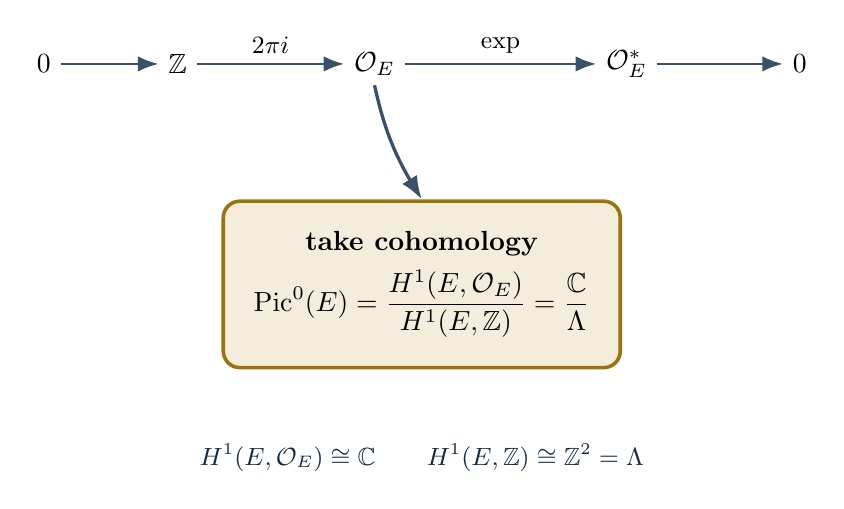
\begin{tikzpicture}[>=Latex]
  % the exponential short exact sequence
  \node (z0) at (0,0)   {$0$};
  \node (Z)  at (1.7,0) {$\Z$};
  \node (O)  at (4.2,0) {$\mathcal{O}_E$};
  \node (Os) at (7.4,0) {$\mathcal{O}_E^{*}$};
  \node (z1) at (9.6,0) {$0$};
  \draw[->, line width=1pt, draw=formslate] (z0)--(Z);
  \draw[->, line width=1pt, draw=formslate] (Z)--node[above, font=\small] {$2\pi i$} (O);
  \draw[->, line width=1pt, draw=formslate] (O)--node[above, font=\small] {$\exp$} (Os);
  \draw[->, line width=1pt, draw=formslate] (Os)--(z1);
  % conclusion box
  \node[draw=formgold!84!black, fill=formgold!15, rounded corners=6pt, line width=1.3pt,
        inner sep=11pt, align=center] (c) at (4.8,-2.8)
    {\textbf{take cohomology}\\[4pt]
     $\Pic^0(E)=\dfrac{H^1(E,\mathcal{O}_E)}{H^1(E,\Z)}=\dfrac{\C}{\Lambda}$};
  \draw[->, line width=1.2pt, draw=formslate] (O.south) to[bend right=10] (c.north);
  \node[font=\small, formteal!55!black, anchor=north] at (4.8,-4.7)
    {$H^1(E,\mathcal{O}_E)\cong\C \qquad H^1(E,\Z)\cong\Z^2=\Lambda$};
\end{tikzpicture}
}
\figcap{$\Pic^0(E)=H^1(\mathcal{O}_E)/H^1(\Z)=\C/\Lambda$; the Hodge piece
$H^{1,0}=\C\,dz$ is Face~1's holomorphic form.}
All such objects are organized by their shape $\tau\in\HH$ modulo $\mathrm{SL}_2(\Z)$, with
global coordinate $j$:
\figH{142pt}{% Moduli: each elliptic curve = a torus C/Lambda = a shape tau in H modulo SL_2(Z).  The
% shaded fundamental domain F is one curve per point; j is the global coordinate on
% H/SL_2(Z).  (Fresh file for the synthesis poster; same look as the main sheet's modular
% figure.)
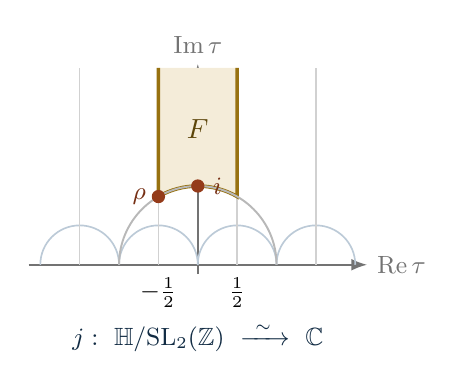
\begin{tikzpicture}[>=Latex]
  \def\rt{0.86603}
  \draw[->, black!55, line width=0.6pt] (-2.15,0)--(2.15,0) node[right, font=\small] {$\operatorname{Re}\tau$};
  \draw[->, black!55, line width=0.6pt] (0,-0.12)--(0,2.55) node[above, font=\small] {$\operatorname{Im}\tau$};
  \foreach \a/\b in {-2/-1,-1/0,0/1,1/2}{
    \pgfmathsetmacro\c{(\a+\b)/2}\pgfmathsetmacro\rr{(\b-\a)/2}
    \draw[formteal!30, line width=0.6pt] (\c+\rr,0) arc[start angle=0, end angle=180, radius=\rr];}
  \foreach \x in {-1.5,-0.5,0.5,1.5}{\draw[black!18, line width=0.5pt] (\x,0)--(\x,2.5);}
  \fill[formgold!16] (-0.5,2.5)--(-0.5,\rt) arc[start angle=120, end angle=60, radius=1]--(0.5,2.5)--cycle;
  \draw[formgold!82!black, line width=1.3pt]
    (-0.5,2.5)--(-0.5,\rt) arc[start angle=120, end angle=60, radius=1]--(0.5,2.5);
  \draw[black!28, line width=0.7pt] (1,0) arc[start angle=0, end angle=180, radius=1];
  \fill[formrust!88!black] (0,1) circle (2.4pt);
  \node[right=2pt, font=\small, formrust!70!black] at (0,1) {$i$};
  \fill[formrust!88!black] (-0.5,\rt) circle (2.4pt);
  \node[left=1pt, font=\small, formrust!70!black] at (-0.5,\rt) {$\rho$};
  \node[formgold!50!black] at (0,1.72) {$F$};
  \node[below, font=\small] at (-0.5,-0.04) {$-\tfrac12$};
  \node[below, font=\small] at (0.5,-0.04) {$\tfrac12$};
  \node[font=\small, formteal!55!black, anchor=north] at (0,-0.6)
    {$j:\ \HH/\mathrm{SL}_2(\Z)\ \xrightarrow{\ \sim\ }\ \C$};
\end{tikzpicture}
}
\figcap{$\HH/\mathrm{SL}_2(\Z)\xrightarrow{\sim}\C$ via the $j$-invariant; $i,\rho$ are the
extra-symmetric curves.}
\callout{formgold}{One object.}{Over $\C$, $\C/\Lambda$, $\Pic^0(E)$ and $E(\C)$ are three
\emph{presentations} of one abelian variety --- not merely isomorphic, but biholomorphic.}}

%========================= COLUMN 3: over F_p and the frontier =========================
\column{0.34}

\block{\large \textbf{4.} Specialize: over $\F_p$, the frontier}{%
\normalsize
The group law is rational, so $E$ makes sense over any field. Over a finite field the three
faces collapse to a finite group --- and a new world opens.
\par\smallskip
\textbf{Finite fields \& Hasse.} $E(\F_p)$ is a finite abelian group with
$\#E(\F_p)=p+1-a_p$, $|a_p|\le 2\sqrt p$: a band of width $4\sqrt p$ about $p+1$. (For
$y^2=x^3+2x+1$, $E(\F_{13})$ is cyclic of order $8$.)
\figH{206pt}{% Hasse: #E(F_p) = p+1-a_p with |a_p| <= 2 sqrt p, so every count lands in the band of
% width 4 sqrt p about p+1.  Real data for y^2 = x^3 - x + 1 over primes 5..89
% (computed in python); all dots fall inside the shaded band.
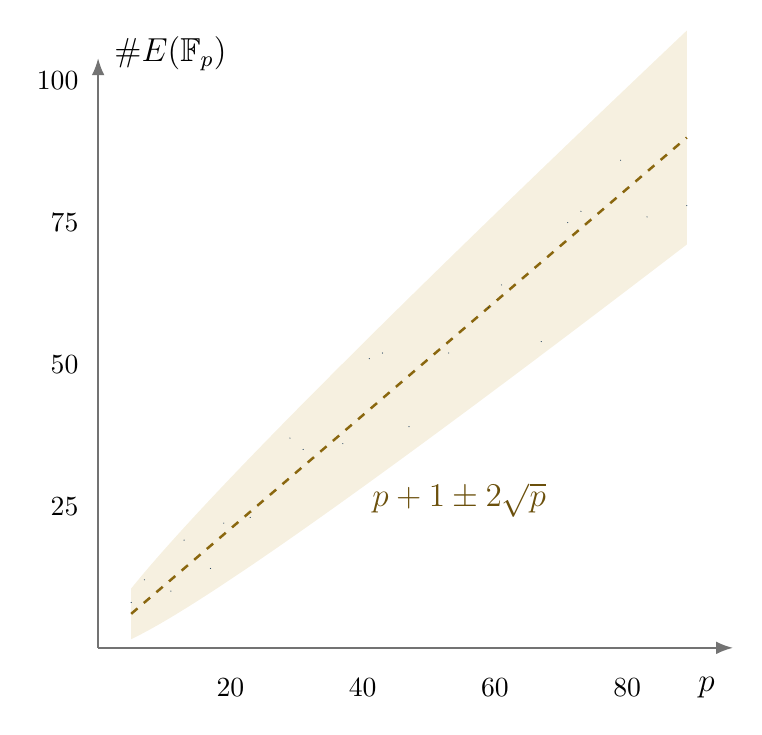
\begin{tikzpicture}[>=Latex, xscale=0.084, yscale=0.072]
  % the Hasse band  p+1 ± 2 sqrt p
  \fill[formgold!13]
    plot[domain=5:89, samples=60] (\x,{\x+1+2*sqrt(\x)}) --
    plot[domain=89:5, samples=60] (\x,{\x+1-2*sqrt(\x)}) -- cycle;
  % centre line p+1
  \draw[formgold!75!black, dashed, line width=0.9pt, domain=5:89, samples=40]
    plot (\x,{\x+1}) ;
  % axes
  \draw[->, black!55, line width=0.7pt] (0,0)--(96,0);
  \draw[->, black!55, line width=0.7pt] (0,0)--(0,104);
  \node[font=\large] at (92,-7) {$p$};
  \node[font=\large, anchor=south west] at (1,100) {$\#E(\F_p)$};
  % data points
  \foreach \p/\n in {5/8,7/12,11/10,13/19,17/14,19/22,23/23,29/37,31/35,37/36,41/51,
                     43/52,47/39,53/52,59/60,61/64,67/54,71/75,73/77,79/86,83/76,89/78}{
    \fill[formteal!70!black] (\p,\n) circle (2.6pt);}
  \node[font=\large, formgold!58!black, anchor=west] at (40,26) {$p+1\pm 2\sqrt p$};
  \foreach \p in {20,40,60,80}{\node[font=\normalsize] at (\p,-7) {$\p$};}
  \foreach \n in {25,50,75,100}{\node[font=\normalsize, anchor=east] at (-1.5,\n) {$\n$};}
\end{tikzpicture}
}
\figcap{Real counts $\#E(\F_p)$ for $y^2=x^3-x+1$, $p\le 89$: all inside the Hasse band
$p+1\pm2\sqrt p$.}
\textbf{Cryptography.} Adding is fast but \emph{dividing} is not: recovering $n$ from $nP$
is the elliptic-curve discrete logarithm, the hardness behind ECC and ECDSA.
\par\smallskip
\textbf{Galois and the Tate module.} The torsion $E[\ell^n]$ carries a
$\operatorname{Gal}(\overline\Q/\Q)$-action --- the curve's arithmetic genome.
\figH{214pt}{% The Tate module and the Galois representation, stacked vertically.  The torsion
% E[l^n]=(Z/l^n)^2 forms an inverse system under x l; its limit is T_l E = Z_l^2, on which
% the absolute Galois group acts, giving  rho : Gal(Qbar/Q) -> GL_2(Z_l).
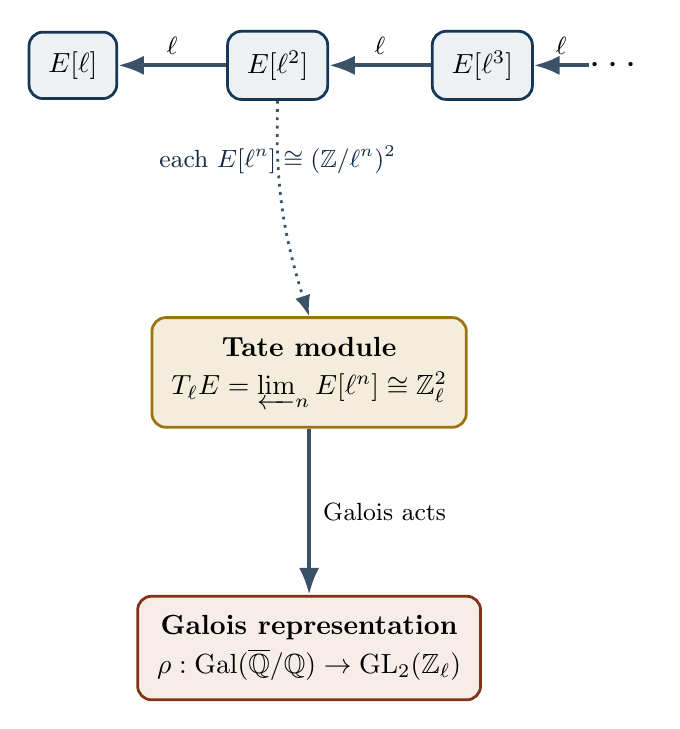
\begin{tikzpicture}[>=Latex,
    tb/.style={rectangle, rounded corners=5pt, draw=formteal!70!black, line width=1pt,
      fill=formteal!8, inner sep=7pt, align=center}]
  % inverse system (top row)
  \node[tb] (e1) at (0,0)   {$E[\ell]$};
  \node[tb] (e2) at (2.6,0) {$E[\ell^2]$};
  \node[tb] (e3) at (5.2,0) {$E[\ell^3]$};
  \node[font=\Large] at (6.9,0) {$\cdots$};
  \draw[<-, line width=1.4pt, draw=formslate] (e1)--node[above, font=\small] {$\ell$} (e2);
  \draw[<-, line width=1.4pt, draw=formslate] (e2)--node[above, font=\small] {$\ell$} (e3);
  \draw[<-, line width=1.4pt, draw=formslate] (e3)--node[above, font=\small] {$\ell$} (6.55,0);
  \node[font=\small, formteal!55!black, anchor=north] at (2.6,-0.9)
    {each $E[\ell^n]\cong(\Z/\ell^n)^2$};
  % Tate module (middle), centred
  \node[tb, draw=formgold!84!black, fill=formgold!15] (T) at (3.0,-3.9)
    {\textbf{Tate module}\\[2pt]$T_\ell E=\varprojlim_n E[\ell^n]\cong\Z_\ell^{2}$};
  \draw[->, dotted, line width=1pt, draw=formslate] (e2.south) to[bend right=10] (T.north);
  % Galois representation (bottom), centred
  \node[tb, draw=formrust!76!black, fill=formrust!10] (G) at (3.0,-7.4)
    {\textbf{Galois representation}\\[2pt]$\rho:\operatorname{Gal}(\overline{\Q}/\Q)\to\mathrm{GL}_2(\Z_\ell)$};
  \draw[->, line width=1.5pt, draw=formslate] (T)--node[right=1pt, font=\small] {Galois acts} (G);
\end{tikzpicture}
}
\figcap{The torsion levels form an inverse system; its limit $T_\ell E\cong\Z_\ell^2$ carries
$\rho:\operatorname{Gal}(\overline\Q/\Q)\to\mathrm{GL}_2(\Z_\ell)$.}
\textbf{Modularity, BSD, CM.} Every $E/\Q$ is \emph{modular} (Wiles --- the theorem behind
Fermat); the rank of $E(\Q)$ is governed by Birch--Swinnerton-Dyer; and CM curves (like
$y^2=x^3-x$, $j=1728$) tie to class field theory.
\callout{formteal}{One identity, two worlds.}{Over $\C$ the three faces are one geometry;
over $\F_p$ or $\Q$ the same law is arithmetic. The dictionary runs in every direction.}
\par\smallskip
{\footnotesize\textbf{Author:} \(\langle\)Your Name\(\rangle\) \,\textbullet\,
\(\langle\)email\(\rangle\) \,\textbullet\, seeking PhD positions in arithmetic \& algebraic
geometry. \;Companion to the main poster and the gallery.}}

\end{columns}
\end{document}
